\section{Discussion}
\begin{figure}[ht!]
    \centering
    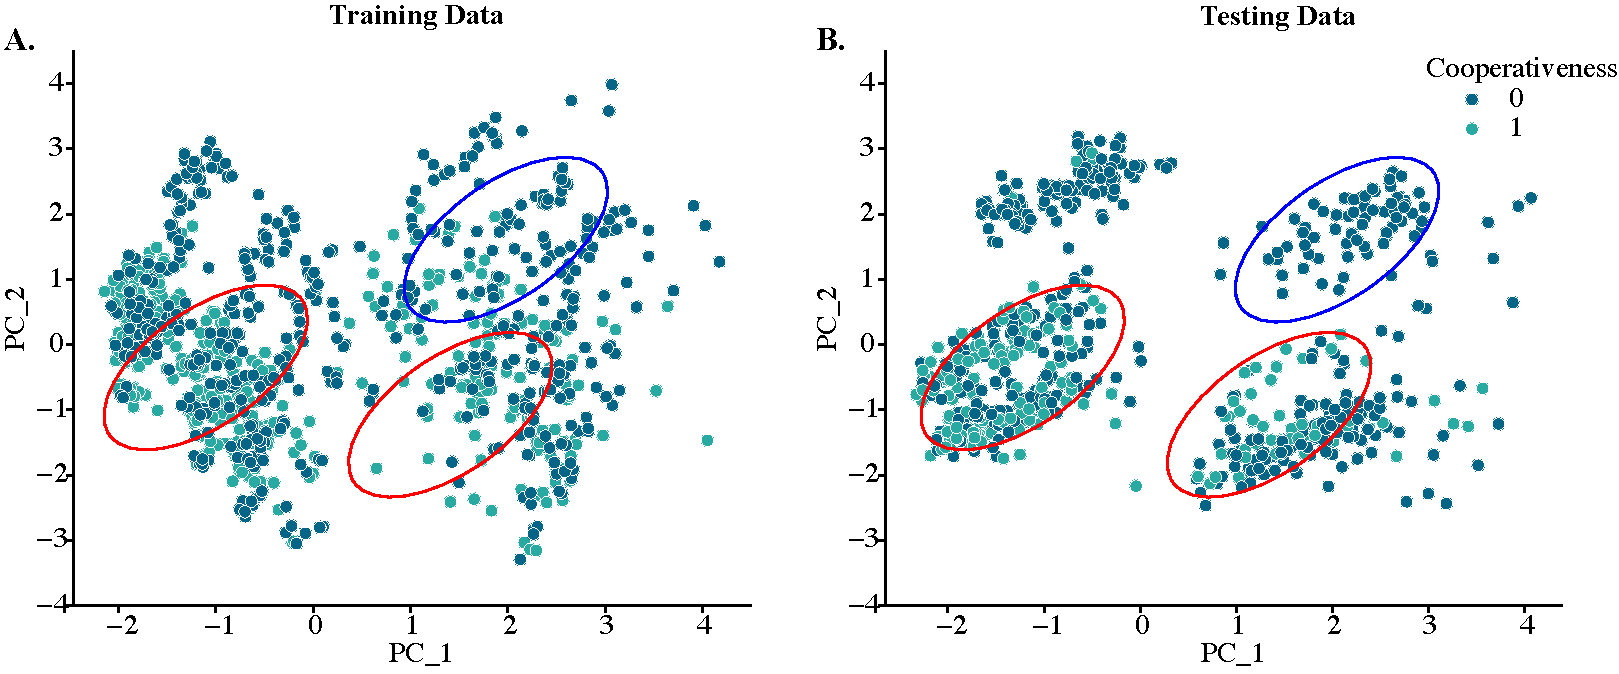
\includegraphics[width=\linewidth]{Figures/Figure6.pdf}
    \caption{Exploration of Accuracy Imbalance. Shown are the scatter plots of untransformed two principal components of (A.) training data and (B.) testing data.}
    \label{fig:figure6}
\end{figure} 

During our preliminary exploration of the data, we clustered the dataset, balancing respect to a respondents preference for civil-liberty or security-based policy. Although there appeared to be underlying trends in the data, the cluster algorithms employed were unable to separate the data on civil-liberty or security-based policy. Our suspicion was that there were untrustworthy samples in the dataset since some clusters were almost pure outside of a few mislabeled samples. Upon further inspection of the dataset, we confirmed our suspicions that some data points were higher fidelity than others. A large number of samples contained low cooperation scores by the interviewer and others completed the survey in unreasonable short time periods. This led us to our current research task of filtering out uncooperative samples in survey datasets to produce high fidelity datasets without sacrificing classification accuracy. 

Next we started developing a classifier to identify samples that contained high levels of cooperation as measured by the interviewer. At this stage we found that our dataset contains a particular form of data bias called batch effect. Batch effect occurs when data variations cause biases that make it challenging to identify the true causes of the relationship at play. In our case the two variables causing the batch effect were RWAVENEW and RWAVEOLD. RWAVENEW denotes if this is the first time a respondent is being surveyed and RWAVEOLD denotes if the respondent is a repeat survey participant. When training classifiers to predict cooperativeness of respondents RWAVENEW and RWAVEOLD drown out the feature importance of all the other features as can be seen in Figure 2. To address the batch effect, we removed both RWAVENEW and RWAVEOLD from our dataset. The result of removing RWAVEOLD and RWAVENEW can be seen in plots A, B, and C of Figure 3. In Figure 3, plots A, B, and C demonstrate more well rounded feature importances than those found in Figure 2. 

After removing the features causing the batch effect, we gathered out baseline feature importance from our classifiers. While these feature importances were more interpretable than our previous feature importances, all three classifiers overfit with respect to attribute W2TOTCL. In each classifier, as depicted in plots A, B, and C of Figure 3, W2TOTCL is by far the most important feature. However, when looking at the data and the context of our investigation this implies that a respondent's cooperation can be predicted based on whether they support civil-liberty based policy or not. Upon another round of inspecting the data, there is a reasonable explanation as to why these classifiers are finding this pattern. In the original dataset, out of those samples who were labeled cooperative, only 18\% answered a question where they favored civil liberties. However, for those respondents who did not take the survey seriously, 45\% of them answered a question where they favored civil liberties. 
	
To address the overfitting we initially faced, we designed a data transformation as described in Data Transformation and applied it to our dataset. Again, like when we removed the batch effect variables, the feature importances became less centralized in the most important features. Notably, two of our three classifiers trained on transformed data did not identify W2TOTCL as the most important feature. However, features strongly related to a particular preference for or against civil liberties policy were consistently influential. Our takeaway is that we continually improved the performance of the model but there is likely still overfitting in our classifiers. 

We explore more on the imbalanced accuracy in the baseline results. Interestingly, 0 which is uncooperative, is the majority class in the testing data, and the the testing accuracy supposes to be higher in uncooperative class. However, the testing accuracy of minority class is significantly higher than the other. We therefore suspect that something unexpected is happening in the feature space for the training and testing data. Through further investigation, first, we found that the testing data created by the stratified train-test split by sklearn can not fully capture the inherent data structure of the training data. From figure ~\ref{fig:figure6}, it is apparent that the train data has two clusters but the testing data has four clusters, where some information between the connection in top and bottom cluster is lost. Second, we discovered that the reason cooperative data is more identifiable in testing data is that they seem to form a cluster themselves in the testing data as indicated by the red circle, where in the training data, these circle contains majority of cooperative class. In addition, as indicated by the blue circle, some of the uncooperative class might be misclassified because in the training data, there are mixed uncooperative and cooperative class, which accounts for the low performance in the uncooperative class.

In benchmarking of data augmentation methods, we found that, data augmentation methods are more effective in training data with low dimensional features, and GAN is more effective with transformed data. We believed that since in low-dimensional data, each feature tends to carry more significance, and there's less noise compared to high-dimensional data, data augmentation in such a setting can effectively introduce meaningful variability without overwhelming the model with noise or irrelevant information. This helps the model learn the essential patterns more effectively. In addition, in high-dimensional spaces, up-sampling or down-sampling becomes much more challenging due to the curse of dimensionality because most of the sampling based data augmentation methods involve calculating distance. Additionally, the purpose of augmenting a GAN after sampling-based augmentation methods is to increase the training size. Therefore, it is reasonable that GAN is more effective in transformed data since from table ~\ref{tab:table1}, data after transformed has significantly less samples after processing compared to the untransformed data. That also accounts for why GAN improves the performance after applying editENN since editENN generates a small training dataset compared to other methods. 